% !Mode:: "TeX:UTF-8"
\title{第二次上机实验报告:单细胞聚类}
\author{江昱峰 21009200038} 
\documentclass {article}
\usepackage[UTF8]{ctex}
\usepackage{graphicx}
\usepackage{float}
\usepackage{hyperref}
\usepackage{makecell}
\begin{document}
	%\begin{sloppypar}
	\maketitle{}	
	\section{背景介绍}
	聚类分析是数据挖掘和分析领域中常用的一种技术,用于将数据集中的对象按照相似性进行分组。聚类分析可以帮助我们发现数据中的隐藏模式、结构和关系,从而对数据进行更深入的理解和分析。
	
	在现实生活和工业实践中,数据集往往包含大量的样本和特征,而且这些数据的结构和关系不容易直观地观察和理解。聚类分析可以帮助我们从复杂的数据集中提取出有意义的信息,发现数据中的群组或簇,并将相似的样本归类到同一个簇中。
	
	聚类分析在各个领域都有广泛的应用。例如,在市场营销中,可以利用聚类分析来识别具有相似购买行为的消费者群体,从而制定针对性的营销策略。在生物学领域,聚类分析可以用于基因表达数据的分类和研究,帮助科学家发现基因的功能和相互作用关系。在社交网络分析中,聚类分析可以用于识别具有相似兴趣和行为的用户群体,从而推荐个性化的内容和服务。
	
	\section{实验目的}
	实验目的是实践并掌握聚类分析有关的内容,具体包括以下 部分:
	\begin{itemize}
		\item 通过差异表达分析、方差筛选等方法进行基因的特征选择;
		\item 通过主成分分析(PCA)、t-SNE等方法进行基因的降维;
		\item 掌握K均值、层次聚类、DBSCAN等聚类算法的原理,并将其应用于基因的聚类;
		\item 基因的聚类结果评估,分为内部、外部指标计算(利用真实标签);
		\item 通过二维或三维降维方法t-SNE、UMAP等进行基因聚类结果的可视化。
	\end{itemize}	
	
	\section{任务描述}
	\begin{enumerate}
		\item 特征选择和降维 \\
		从所有基因中选择最具信息量的基因,例如通过差异表达分析或方差筛选。使用降维方法(如主成分分析(PCA)或t-SNE)将高维数据映射到较低维空间,以便于可视化和聚类。
		\item 聚类算法应用 \\
		选择合适的聚类算法,如层次聚类、DBSCAN等,将细胞分配到不同的聚类簇中。
		\item 聚类结果评估和可视化 \\
		通过内部指标(如轮廓系数)或外部指标(如调整兰德指数ARI)评估聚类结果的质量。使用二维或三维降维方法(如t-SNE、UMAP)对聚类结果进行可视化展示,以便于观察细胞群集的分布和相互作用关系。 
	\end{enumerate}
	
	\section{数据描述}
	单细胞RNA-seq测序数据介绍:
	\begin{enumerate}
		\item Zeisel\_df \\
		预处理过后的单细胞数据集,已经进行了细胞类型筛选。行代表细胞,列代表基因;
		\item Sclabel \\
		Zeisel\_df中细胞对应的真实细胞类型标签。
	\end{enumerate}
	
	\section{实验原理}
	\subsection{主成分分析(PCA)}
	\label{PCA算法原理}
	假设有n个样本,p个指标,则可构成大小为n×p的样本矩阵x:
	\begin{equation}
		\centering
		\mathrm{x}=\left[\begin{array}{cccc}
			\mathrm{x}_{11} & \mathrm{x}_{12} & \cdots & \mathrm{x}_{1 \mathrm{p}} \\
			\mathrm{x}_{21} & \mathrm{x}_{22} & \cdots & \mathrm{x}_{2 \mathrm{p}} \\
			\vdots & \vdots & \ddots & \vdots \\
			\mathrm{x}_{\mathrm{n} 1} & \mathrm{x}_{\mathrm{n} 2} & \cdots & \mathrm{x}_{\mathrm{np}}
		\end{array}\right]=\left(\mathrm{x}_1, \mathrm{x}_2, \cdots, \mathrm{x}_{\mathrm{p}}\right)
	\end{equation}
	
	\begin{enumerate}
		\item 首先对其进行标准化处理:
		\begin{itemize}
			\item 按列计算均值: 
			$\bar{x}_{\mathrm{j}}=\frac{1}{\mathrm{n}} \sum_{\mathrm{i}=1}^{\mathrm{n}} \mathrm{x}_{\mathrm{ij}}$
			
			\item 标准差: $\mathrm{S}_{\mathrm{j}}=\sqrt{\frac{\sum_{\mathrm{i}=1}^{\mathrm{n}}\left(\mathrm{x}_{\mathrm{ij}}-\overline{\mathrm{x}}_{\mathrm{j}}\right)^2}{\mathrm{n}-1}}$
			
			\item 标准化数据: $\mathrm{X}_{\mathrm{ij}}=\frac{\mathrm{x}_{\mathrm{ij}}-\overline{\mathrm{x}}_{\mathrm{j}}}{\mathrm{S}_{\mathrm{j}}}$
			
			\item 原始样本矩阵经过标准化变化: \\
			$\mathrm{X}=\left[\begin{array}{cccc}\mathrm{X}_{11} & \mathrm{X}_{12} & \cdots & \mathrm{X}_{1 \mathrm{p}} \\ \mathrm{X}_{21} & \mathrm{X}_{22} & \cdots & \mathrm{X}_{2 \mathrm{p}} \\ \vdots & \vdots & \ddots & \vdots \\ \mathrm{X}_{\mathrm{n} 1} & \mathrm{X}_{\mathrm{n} 2} & \cdots & \mathrm{X}_{\mathrm{np}}\end{array}\right]=\left(\mathrm{X}_1, \mathrm{X}_2, \cdots, \mathrm{X}_{\mathrm{p}}\right)$
		\end{itemize}
		
		
		\item 计算标准化样本查的协方差矩阵:
		\begin{equation}
			\centering
			\mathbf{R}=\left[\begin{array}{cccc}
				\mathbf{r}_{11} & \mathrm{r}_{12} & \cdots & \mathbf{r}_{1 \mathrm{p}} \\
				\mathbf{r}_{21} & \mathrm{r}_{22} & \cdots & \mathbf{r}_{2 \mathrm{p}} \\
				\vdots & \vdots & \ddots & \vdots \\
				\mathbf{r}_{\mathrm{p} 1} & \mathrm{r}_{\mathrm{p} 2} & \cdots & \mathbf{r}_{\mathrm{pp}}
			\end{array}\right]
		\end{equation}
		
		\begin{equation}
			\centering
			\mathrm{r}_{\mathrm{ij}}=\frac{1}{\mathrm{n}-1} \sum_{\mathrm{k}=1}^{\mathrm{n}}\left(\mathrm{X}_{\mathrm{ki}}-\overline{\mathrm{X}}_{\mathrm{i}}\right)\left(\mathrm{X}_{\mathrm{ki}}-\overline{\mathrm{X}}_{\mathrm{j}}\right)=\frac{1}{\mathrm{n}-1} \sum_{\mathrm{k}=1}^{\mathrm{n}} \mathrm{X}_{\mathrm{ki}} \mathrm{X}_{\mathrm{kj}}
		\end{equation}
		
		\item 计算R的特征值和特征值向量:
		\begin{itemize}
			\item 特征值: $\lambda_1 \geq \lambda_2 \geq \cdots \geq \lambda_{\mathrm{p}} \geq 0, \quad\left({R}\right.$ 是半正定矩阵, 且 $\left.{tr}(R)=\sum_{\mathrm{k}=1}^{\mathrm{p}} \lambda_{\mathrm{k}}=\mathrm{p}\right)$
			
			\item 特征向量: $\mathrm{a}_1=\left[\begin{array}{c}\mathrm{a}_{11} \\ \mathrm{a}_{21} \\ \vdots \\ \mathrm{a}_{\mathrm{p} 1}\end{array}\right], \mathrm{a}_2=\left[\begin{array}{c}\mathrm{a}_{12} \\ \mathrm{a}_{22} \\ \vdots \\ \mathrm{a}_{\mathrm{p} 2}\end{array}\right], \cdots, \mathrm{a}_{\mathrm{p}}=\left[\begin{array}{c}\mathrm{a}_{1 \mathrm{p}} \\ \mathrm{a}_{2 \mathrm{p}} \\ \vdots \\ \mathrm{a}_{\mathrm{pp}}\end{array}\right]$
		\end{itemize}
		
		\item 计算主成分共享率以及累计贡献率:\\
		贡献率 $=\frac{\lambda_{\mathrm{i}}}{\sum_{\mathrm{k}=1}^{\mathrm{p}} \lambda_{\mathrm{k}}}$, 累加贡献率 $=\frac{\sum_{\mathrm{k}=1}^{\mathrm{i}} \lambda_{\mathrm{k}}}{\sum_{\mathrm{k}=1}^{\mathrm{p}} \lambda_{\mathrm{k}}}, \quad(\mathrm{i}=1,2, \cdots, \mathrm{p})$
		
		\item 写出主成分:\\
		一般取累计贡献率超过 $80 \%$ 的特征值所对应的第一、第二、 $\ldots$ 第 $m(m \leq p)$ 个主成分。
		第 $\mathrm{i}$ 个主成分: $\mathrm{F}_{\mathrm{i}}=\mathrm{a}_{1 \mathrm{i}} \mathrm{X}_1+\mathrm{a}_{2 \mathrm{i}} \mathrm{X}_2+\cdots+\mathrm{a}_{\mathrm{pi}} \mathrm{X}_{\mathrm{p}}$
		
		\item 根据系数分析主成分代表的意义:\\
		对于某个主成分而言,指标前面的系数越大,代表该指标对于该主成分的影响越大。
		
	\end{enumerate}
	
	\subsection{Leiden算法}
	\label{Leiden算法原理}
	Leiden算法步骤伪代码如下图所示:
	\begin{table}[H]
		\centering
		\caption{Leiden算法伪代码}
		\begin{tabular}{rl}
			\hline
			序号 & {具体步骤}\\ \hline
			1:& \textbf{function} LeIDEN(Graph $G$, Partition $\mathcal{P}$ ) \\
			2: & \quad \textbf{do} \\
			3: & \qquad $\mathcal{P} \leftarrow {MovenodesFast}(G, \mathcal{P})$ \\
			4: & \qquad done $\leftarrow|\mathcal{P}|=|V(G)|$ \\
			5: & \qquad \textbf{if} not done \textbf{then} \\
			6: & \qquad \quad $\mathcal{P}_{ {refined }} \leftarrow$ RefinePartition $(G, \mathcal{P})$ \\
			7: & \qquad \quad $G \leftarrow {AggregateGraph}\left(G, \mathcal{P}_{ {refined }}\right)$ \\
			8: & \qquad \quad $\mathcal{P} \leftarrow\{\{v \mid v \subseteq C, v \in V(G)\} \mid C \in \mathcal{P}\}$ \\
			9: & \qquad \textbf{end if} \\
			10: & \quad \textbf{while} not done \\
			11: & \quad \textbf{return} flat ${ }^*(\mathcal{P})$ \\
			12: & \textbf{end function} \\
		\end{tabular}
	\end{table}	

	\begin{table}[H]
		\centering
		\begin{tabular}{rl}
			13: & \textbf{function} MoveNodesFast(Graph $G$, Partition $\mathcal{P}$ ) \\
			14: & \quad $Q \leftarrow {QUeUE}(V(G))$ \\
			15: & \quad \textbf{do} \\
			16: & \qquad $v \leftarrow Q$.remove() \\
			17: & \qquad $C^{\prime} \leftarrow \arg \max _{C \in \mathcal{P} \cup \emptyset} \Delta \mathcal{H}_{\mathcal{P}}(v \mapsto C)$ \\
			18: & \qquad \textbf{if} $\Delta \mathcal{H}_P\left(v \mapsto C^{\prime}\right)>0$ \textbf{then} \\
			19: & \qquad \quad $v \mapsto C^{\prime}$ \\
			20: & \qquad \quad $N \leftarrow\left\{u \mid(u, v) \in E(G), u \notin C^{\prime}\right\}$ \\
			21: & \qquad \quad $Q . {add}(N-Q)$ \\
			22: & \qquad \textbf{end if} \\
			23: & \quad \textbf{while} $Q \neq \emptyset$ \\
			24: & \textbf{return} $\mathcal{P}$ \\
			25: & \textbf{end function} \\
			\\
			26: & \textbf{function} RefinePartition(Graph $G$, Partition $\mathcal{P}$ ) \\
			27: & \quad $\mathcal{P}_{ {refined }} \leftarrow$ SingletonPartition $(G)$ \\
			28: & \quad \textbf{for} $C \in \mathcal{P}$ \textbf{do} \\
			29: & \qquad $\mathcal{P}_{ {refined }} \leftarrow$ MergenodesSubset $\left(G, \mathcal{P}_{ {refined }}, C\right)$ \\
			30: & \quad \textbf{end for} \\
			31: & \quad \textbf{return} $\mathcal{P}_{ {refined }}$ \\
			32: & \textbf{end function} \\
			\\
			33: & \textbf{function} MergeNodesSubset(Graph $G$, Partition $\mathcal{P}$, Subset $S$ ) \\
			34: & \quad $R=\{v \mid v \in S, E(v, S-v) \geq \gamma\|v\| \cdot(\|S\|-\|v\|)\}$ \\
			35: & \quad \textbf{for} $v \in R$ \textbf{do} \\
			36: & \qquad \textbf{if} $v in singleton community \textbf{then}$ \\
			37: & \qquad \quad $\mathcal{T} \leftarrow\{C \mid C \in \mathcal{P}, C \subseteq S, E(C, S-C) \geq \gamma\|C\| \cdot(\|S\|-\|C\|)\}$ \\
			38: & \qquad \quad ${Pr}\left(C^{\prime}=C\right) \sim\left\{\begin{array}{ll}\exp \left(\frac{1}{\theta} \Delta \mathcal{H}_p(v \mapsto C)\right) & { if } \Delta \mathcal{H}_P(v \mapsto C) \geq 0 \\ 0 & { otherwise }\end{array} \quad\right.$ for $C \in \mathcal{T}$\\
			39: & \qquad \quad $v \mapsto C^{\prime}$ \\
			40: & \qquad \textbf{end if} \\
			41: & \quad \textbf{end for} \\
			42: & \quad \textbf{return} $\mathcal{P}$ \\
			43: & \textbf{end function} \\
		\end{tabular}
	\end{table}	
	
	\begin{table}[H]
		\centering
		\begin{tabular}{rl}	   
			44: & \textbf{function} AggregateGraph(Graph $G$, Partition $\mathcal{P}$ ) \\
			45: & \quad $V \leftarrow \mathcal{P}$ \\
			46: & \quad $E \leftarrow\{(C, D) \mid(u, v) \in E(G), u \in C \in \mathcal{P}, v \in D \in \mathcal{P}\}$ \\
			47: & \quad \textbf{return} Graph $(V, E)$ \\
			48: & \textbf{end function} \\
			\\
			49: & \textbf{function} SingletonPartition(Graph $G)$ \\
			50: & \quad \textbf{return} $\{\{v\} \mid v \in V(G)\}$ \\
			51: & \textbf{end function} \\
			\hline
		\end{tabular}
	\end{table}	
	
	\subsection{聚类指标}
	聚类的混淆矩阵如下表所示:
	\begin{table}[H]
		\centering
		\caption{聚类混淆矩阵}
		\begin{tabular}{|c|c|c|}
			\hline 
			\hspace*{1in} & 同簇 & 非同簇 \\
			\hline 同类 & $\mathrm{TP}$ & $\mathrm{FN}$ \\
			\hline 非同类 & $\mathrm{FP}$ & $\mathrm{TN}$ \\
			\hline
		\end{tabular}
	\end{table}
	
	基于此混淆矩阵,实验中涉及的聚类指标(分为内部、外部指标两类)的名称、含义与计算公式如下所示:
	
	内部聚类指标:
	\begin{table}[H]
		\centering
		\caption{内部聚类指标名称、含义与计算公式}
		\begin{tabular}{ccl}
			\hline
			聚类指标 & 意义 & 计算公式 \\
			\hline
			轮廓系数(SC) & 样本到簇内样本与最近簇距离比 & \makecell{$s=\frac{1}{n} \sum_{i=1}^n s(i)$,\\ 其中$s(i)=\frac{b(i)-a(i)}{\max \{a(i), b(i)\}}$} \\
			DBi指数 & 每个簇与其最相似簇的相似度 & \makecell{$D B=\frac{1}{K} \sum_{i, j=1}^K \max _{i \neq j} R_{i j}$,\\ 其中$R_{i j}=\frac{s_i+s_j}{d_{i j}}$} \\
			CH指数 & 簇间距离与簇内距离的比值 & $s=\frac{B}{K-1} / \frac{W}{n-K}=\frac{B}{W} \cdot \frac{n-K}{K-1}$ \\
			\hline 	                                                                                         
		\end{tabular}
	\end{table}
	
	外部聚类指标:
	\begin{table}[H]
		\centering
		\caption{外部聚类指标名称、含义与计算公式}
		\begin{tabular}{ccl}
			\hline
			聚类指标 & 意义 & 计算公式 \\
			\hline
			RI & 结果一致性 & $R I=\frac{T P+T N}{T P+F P+F N+T N}$ \\
			ARI & 考虑随机分类影响 & $A R I=\frac{2 \times(T P \cdot T N-F N \cdot F P)}{(T P+F N)(F N+T N)+(T P+F P)(F P+T N)}$ \\
			MI & 结果相关性 & $\mathrm{MI}(\mathrm{U}, \mathrm{V})=\sum_{\mathrm{i}=1}^{\mathrm{R}} \sum_{\mathrm{j}=1}^{\mathrm{C}} \mathrm{p}_{\mathrm{i}, \mathrm{j}} \log \left(\frac{\mathrm{p}_{\mathrm{i}, \mathrm{j}}}{\mathrm{p}_{\mathrm{i}} \times \mathrm{p}_{\mathrm{j}}}\right)$ \\
			AMI & 考虑随机分类影响 & ${AMI}(\mathrm{U}, \mathrm{V})=\frac{\mathrm{MI}(\mathrm{U}, \mathrm{V})-{E}\{\mathrm{MI}(\mathrm{U}, \mathrm{V})\}}{\mathrm{F}(\mathrm{H}(\mathrm{U}), \mathrm{H}(\mathrm{V}))-{E}\{\mathrm{MI}(\mathrm{U}, \mathrm{V})\}}$ \\
			NMI & 互信息分数标准化 & ${NMI}(\mathrm{U}, \mathrm{V})=\frac{\mathrm{MI}(\mathrm{U}, \mathrm{V})}{\mathrm{F}(\mathrm{H}(\mathrm{U}), \mathrm{H}(\mathrm{V}))}$ \\
			FMI & 细胞分到同簇概率 & $\mathrm{FMI}=\frac{\mathrm{TP}}{\sqrt{(\mathrm{TP}+\mathrm{FP})(\mathrm{TP}+\mathrm{FN})}}$ \\
			纯度 & 结果中每簇为同类程度 & $Purity=\sum_{\mathrm{i}=1}^{\mathrm{k}} \frac{\mathrm{m}_{\mathrm{i}}}{\mathrm{m}} \mathrm{p}_{\mathrm{i}}$ \\
			精确度 & 正确细胞比例 & Precision $=\frac{T P}{T P+F P}$ \\
			准确度 & 正样本中实际也是比例 & $ACC=\frac{\sum_{i=1}^n \delta\left(s_i, {map}\left(r_i\right)\right)}{n}$ \\
			召回率 & 真实分类中正确细胞比例 & $Recall=\frac{T P}{T P+F N}$ \\
			F1 score & 综合准确性和召回率 & $F$-score $=\frac{2 { Precision } * { Recall }}{{ Precision }+ { Recall }}$ \\
			Jaccard系数 & 结果相似性 & $Jaccard=\frac{T P}{T P+F N+T N}$ \\
			\hline 	                                                                                         
		\end{tabular}
	\end{table}
	
	\subsection{KM(Kuhn-Munkres)算法}
	\label{KM算法原理}
	KM算法步骤如下:
	\begin{enumerate}
		\item 初始化可行顶标的值;
		\item 用匈牙利算法寻找完备匹配;
		\item 若未找到完备匹配则修改可行顶标的值;
		\item 重复步骤2、3直到找到相等子图的完备匹配为止。
	\end{enumerate}
	
	其中,匈利亚算法步骤如下:
	\begin{enumerate}
		\item 置M(无向图G的一个匹配)为空;
		\item 找出一条增广路径P,通过异或操作获得更大的匹配M'代替M;
		\item 重复步骤2直到找不出增广路径为止。
	\end{enumerate}
	
	\section{实验环境}
	本次实验的实验环境见下表:
	\begin{table}[H]
		\caption{实验环境}
		\centering
		\begin{tabular}{cc}
			\hline
			类型 & 工具配置 \\ \hline
			操作系统 & AWS(亚马逊云)服务器- Linux(Ubuntu 20.04)  \\
			编程语言 & Python 3.10(Anaconda 2023 - Jupyter Notebook) \\ 
			编译器  & VScode                                      \\ \hline
		\end{tabular}
	\end{table}
	
	\section{分析步骤}
	第一步当然是数据读取。我用pandas库的read\_csv函数对CSV文件数据进行读取操作。
	
	由于已经进行过数据预处理,此处便直接进入数据分析步骤。
	
	\subsection{特征选择和降维}
	在进行聚类分析步骤之前,为了便于可视化和聚类,我先对数据进行了特征选择和降维操作。
	前半步骤中,我通过方差筛选方法从所有基因中选择最具信息量的基因。
	后半步骤中,在常用的降维算法主成分分析(PCA)、t-SNE(t-随机邻近嵌入)、均匀流形近似和投影(UMAP)、线性判别分析(LDA)、因子分析(FC)、独立分量分析(ICA)、等度量映射(ISOMAP)、局部线性嵌入(LLE)等中,我选择了最为典型、使用广泛的主成分分析(PCA)算法将高维数据映射到较低维空间,具体步骤见\hyperref[PCA算法原理]{对应的实验原理部分}。
	
	\subsection{聚类算法应用}
	接下来开始正式的聚类算法应用步骤。首先需要选择合适的聚类算法。由于单细胞基因表达数据没有明显的密度、层次等差异特征,也并不要求最终聚类成不同层次,同时为了能够选择更好的初始质心,从而提高算法的收敛速度、降低陷入局部最优解的风险、显著的改善分类结果的最终误差,我决定选择Leiden算法。然后,我计算了邻域图,并将图形嵌入二维。接着,我通过Leiden算法进行聚类分析,从而将细胞分配到不同的聚类簇中,具体步骤见\hyperref[Leiden算法原理]{对应的实验原理部分}。
	
	\subsection{聚类结果评估和可视化}
	最后,得到聚类结果后,我对其进行了评估和可视化。我先用KM(Kuhn-Munkres)算法在聚类分析结果标签与真实标签之间建立映射,得到与真实标签关联后的聚类标签,具体步骤见\hyperref[KM算法原理]{对应的实验原理部分}。然后,我根据此聚类标签计算了一些聚类指标,分为如下两类:内部指标,包括轮廓系数(SC,Silhouette Coefficient Index)、DB[i]指数(Davies-Bouldin Index,戴维森堡丁指数)、CH(Calinski-Harabaz 指数,又称方差比准则);外部指标(需结合真实标签),除了常见的RI(兰德系数)、ARI(调整兰德系数)、MI(互信息分数)、NMI(标准化互信息分数)、AMI(调整互信息分数)、FMI(Fowlkes–Mallows指数)之外,还包括课本中簇有效性的面向分类的度量(熵、纯度Purity、精确度Precesion、召回率Recall、F度量)和面向相似性的度量(Jaccard系数)等等。除此之外,其实还有一些内部指标,如紧密度(Compactness)、分割度(Seperation)、邓恩指数(DVI)、SSE(误差平方和)、NCC(Internal and external validation measures)等等。
	最后,我使用二维降维方法UMAP对聚类结果进行可视化展示,进一步计算了每类细胞的标记基因并可视化,绘制了标记基因对气泡图、小提琴图等等,从而观察细胞群集的分布和相互作用关系。
	
	\section{实验结果与可视化}
	\subsection{特征选择和降维}
	主成分分析(PCA)降维结果如下图所示:
	\begin{figure}[H]
		\centering
		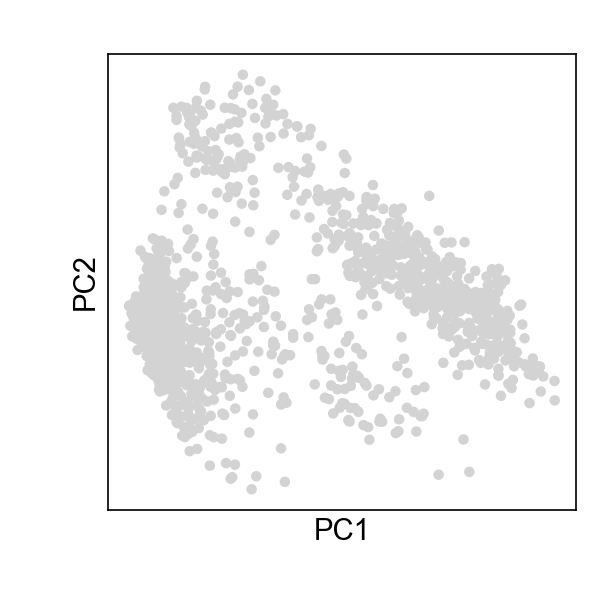
\includegraphics[width=2.5in,height=2.5in]{figures/fig1.png}
		\caption{PCA散点图}
	\end{figure}
	
	\begin{figure}[H]
		\centering
		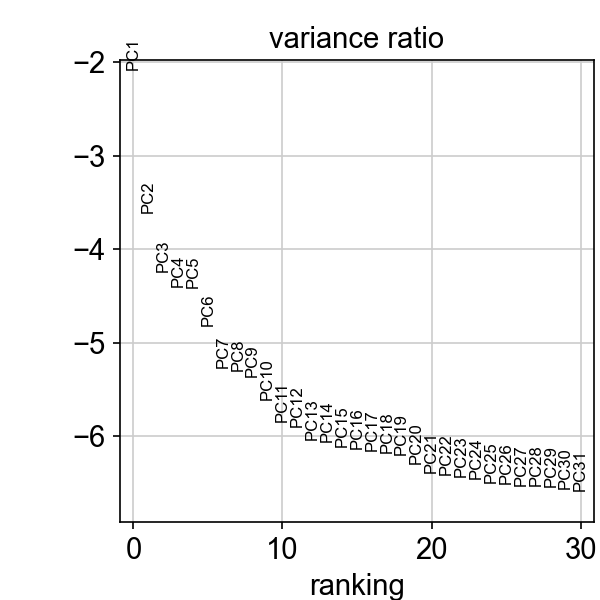
\includegraphics[width=2.5in,height=2.5in]{figures/fig2.png}
		\caption{单个PC对数据总方差的贡献}
	\end{figure}
	
	\subsection{聚类算法应用}
	聚类算法应用得到了17类细胞,聚类邻域图如下图所示:
	\begin{figure}[H]
		\centering
		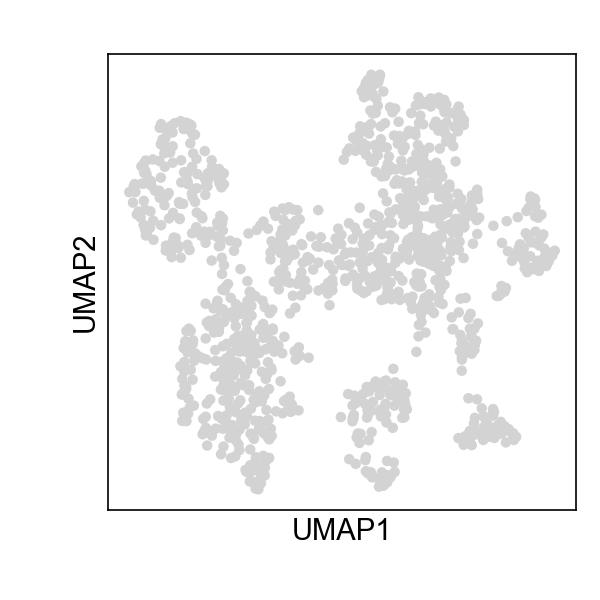
\includegraphics[width=3in,height=3in]{figures/fig3.png}
		\caption{leiden聚类邻域图}
	\end{figure}
	
	聚类标签、结果矩阵(未标记细胞类型)的h5ad文件见实验结果目录。
	
	\subsection{聚类结果评估和可视化}
	聚类指标计算结果如下所示:
	\begin{table}[H]
		\centering
		\caption{内部指标计算结果}
		\begin{tabular}{cc}
			\hline
			聚类指标 & 计算结果 \\
			\hline
			轮廓系数(SC,Silhouette Coefficient Index) & 0.997 \\
			DBi指数(Davies-Bouldin Index,戴维森堡丁指数)& 6.151 \\
			CH(Calinski-Harabaz 指数,又称方差比准则) & 15.583 \\
			\hline                                                                               
		\end{tabular}
	\end{table}
	
	\begin{table}[H]
		\centering
		\caption{外部指标计算结果}
		\begin{tabular}{cc}
			\hline
			聚类指标 & 计算结果 \\
			\hline
			RI(兰德系数) & 0.732 \\
			ARI(调整兰德系数) & 0.779 \\
			MI(互信息分数) & 0.779 \\
			AMI(调整互信息分数) & 0.549 \\
			NMI(标准化互信息分数) & 0.563 \\
			FMI(Fowlkes–Mallows指数) & 0.405 \\
			Purity(纯度) & 92.217\% \\
			Precision(精确度) & 91.817\% \\
			ACC(准确度) & 88.409\% \\
			Recall(召回率) & 96.435\% \\
			F1 score(F度量) & 0.968 \\
			Jaccard系数 & 0.982 \\
			\hline                                                                               
		\end{tabular}
	\end{table}
	
	每类细胞标记基因计算结果:
	
	17类细胞的标记基因分别为``Ccl27a\_loc1''、``Ryr2''、``Wfs1''、``Ttr''、``Reln''、``2610001J05Rik''、``Mog''、``Gpr17''、``Vip''、``Itm2a\_1''、``Metrn''、``Itgb4''、``Itm2a\_2''、``Aqp4''、``Nxph3''、``Tyrobp''、``Lyz2''。
	\begin{figure}[H]
		\centering
		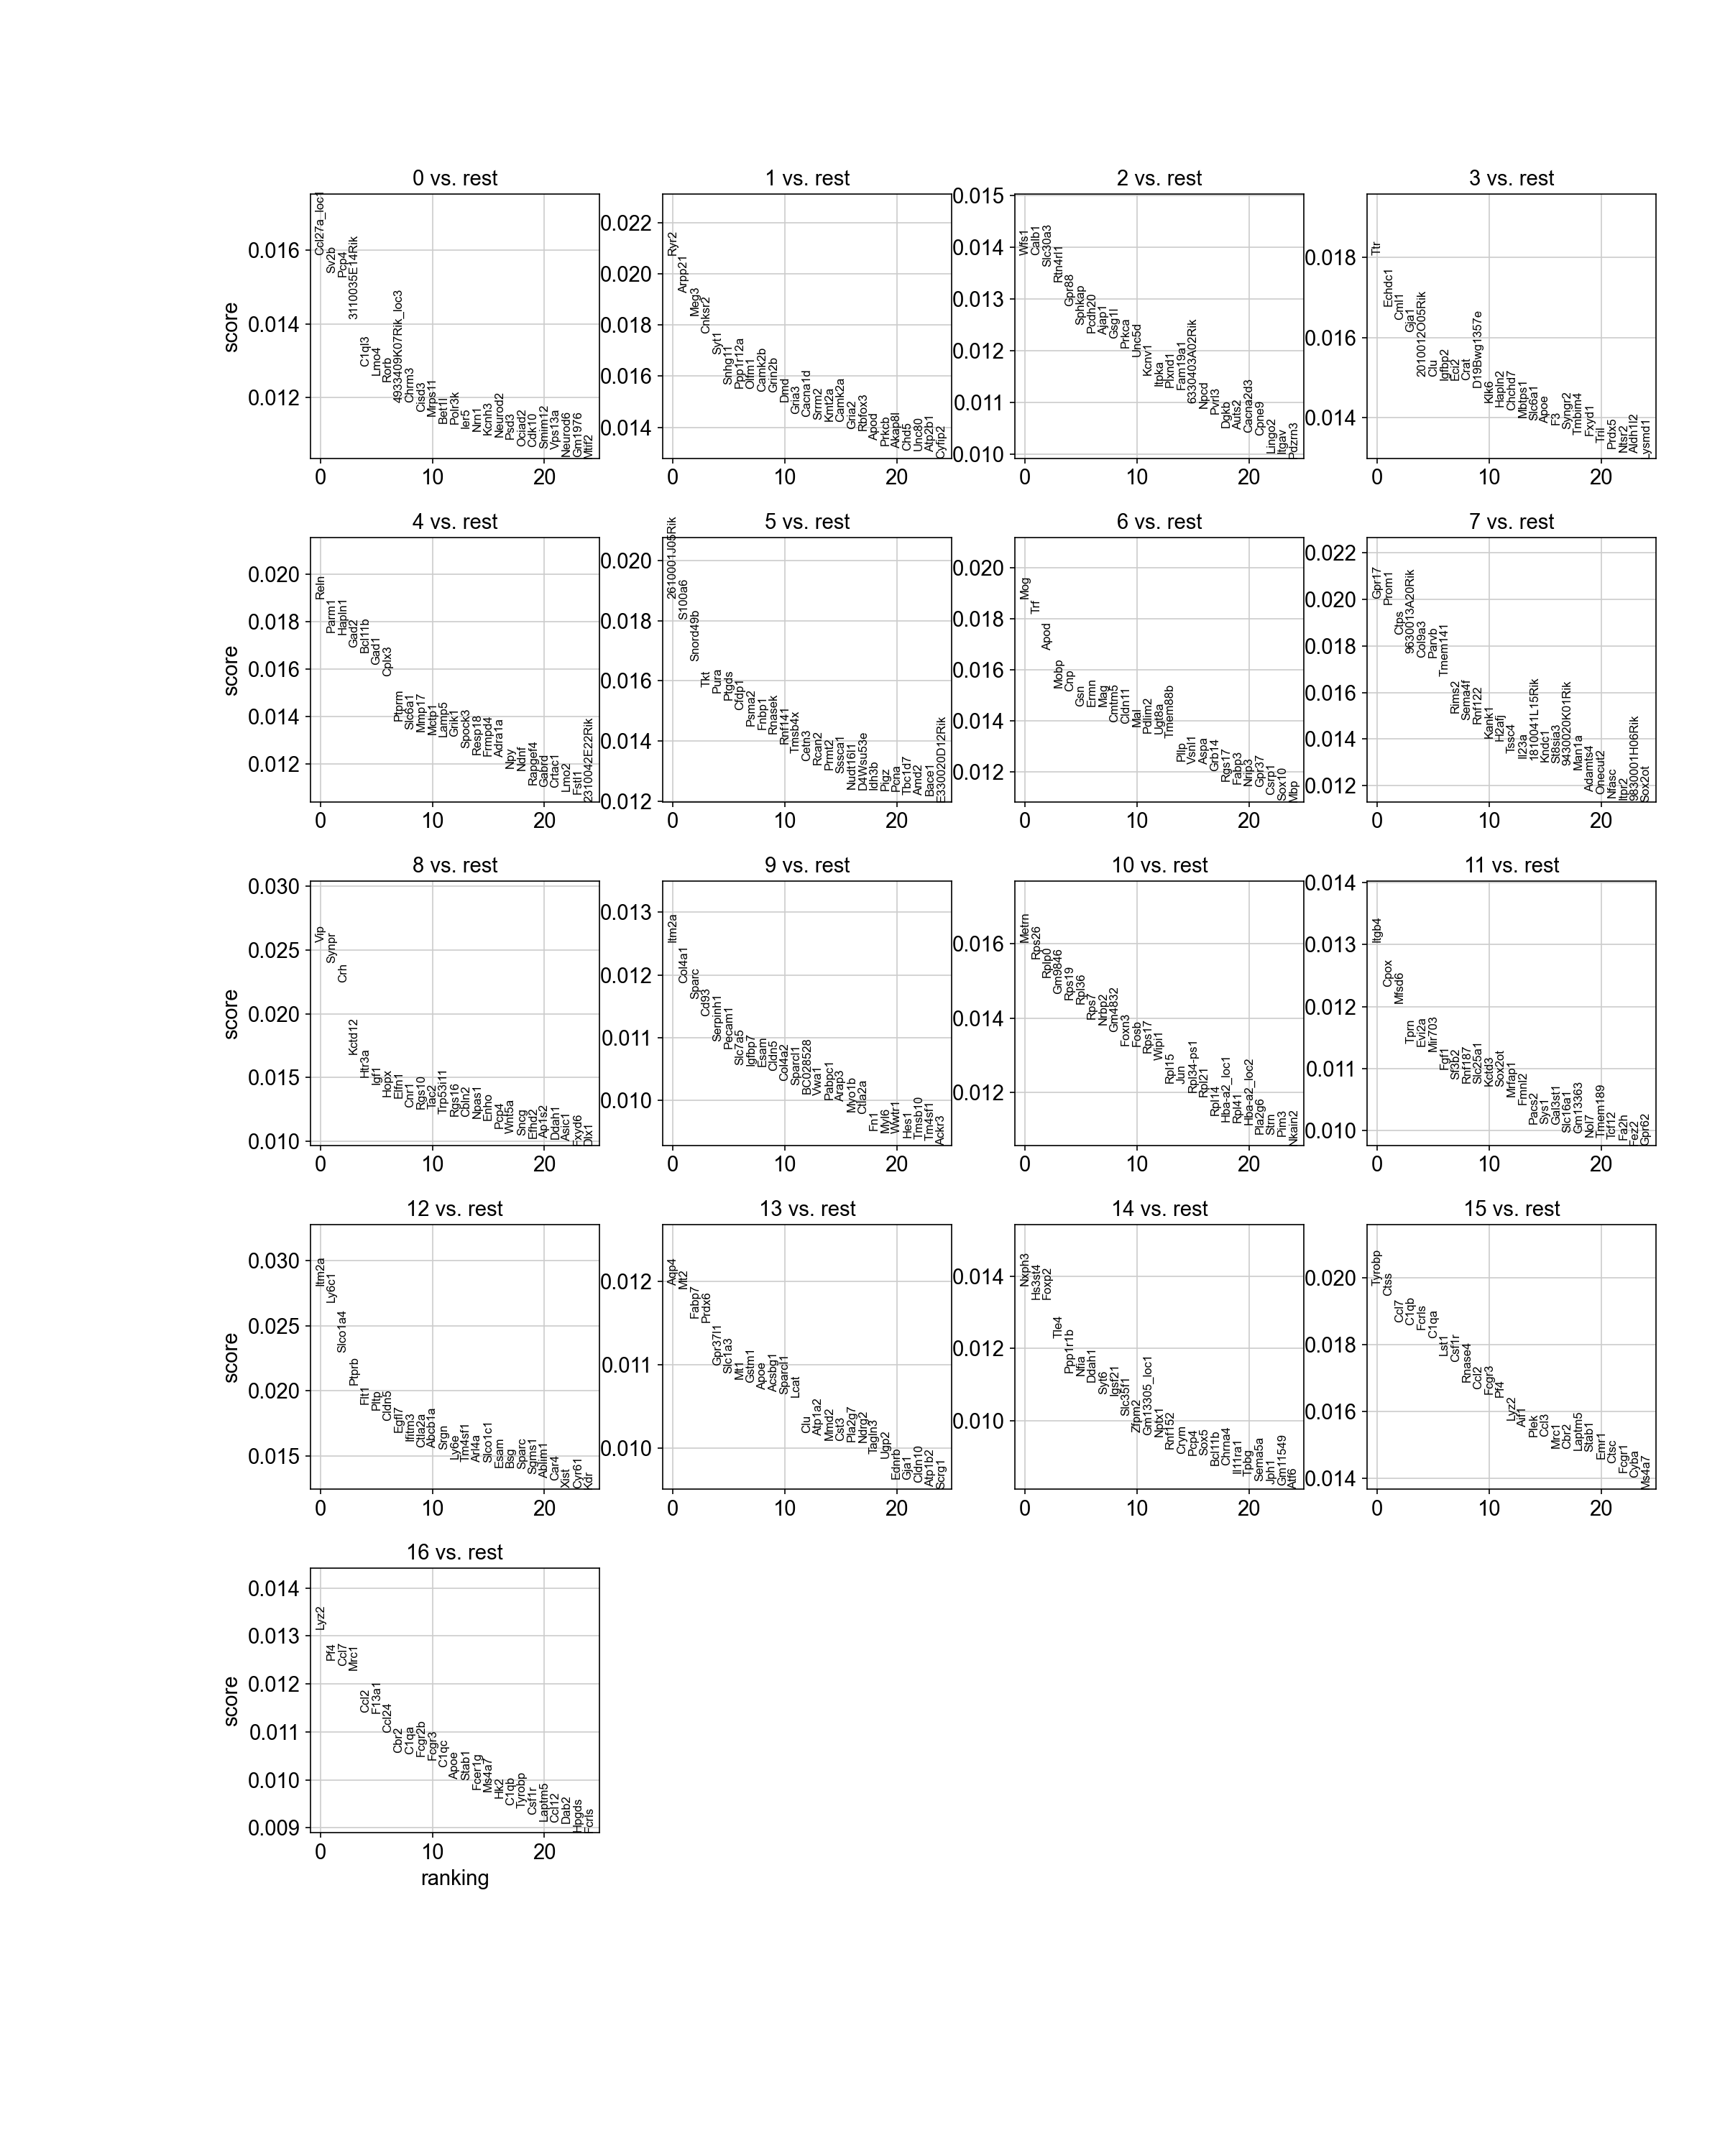
\includegraphics[width=4.5in,height=5.5in]{figures/fig4.png}
		\caption{每个簇中高度差异基因排名}
	\end{figure}
	
	二维降维方法UMAP对聚类结果进行的可视化展示如下所示:
	\begin{figure}[H]
		\centering
		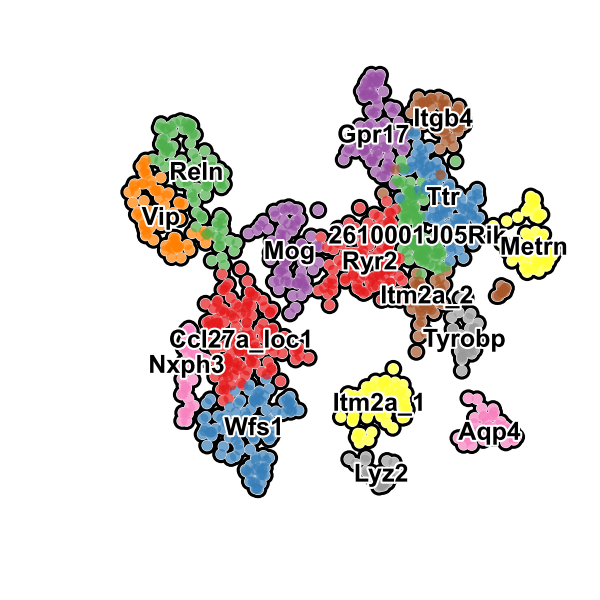
\includegraphics[width=2.5in,height=2.5in]{figures/fig5.png}
		\caption{聚类结果散点图(标记细胞类型)}
	\end{figure}
	
	\begin{figure}[H]
		\centering
		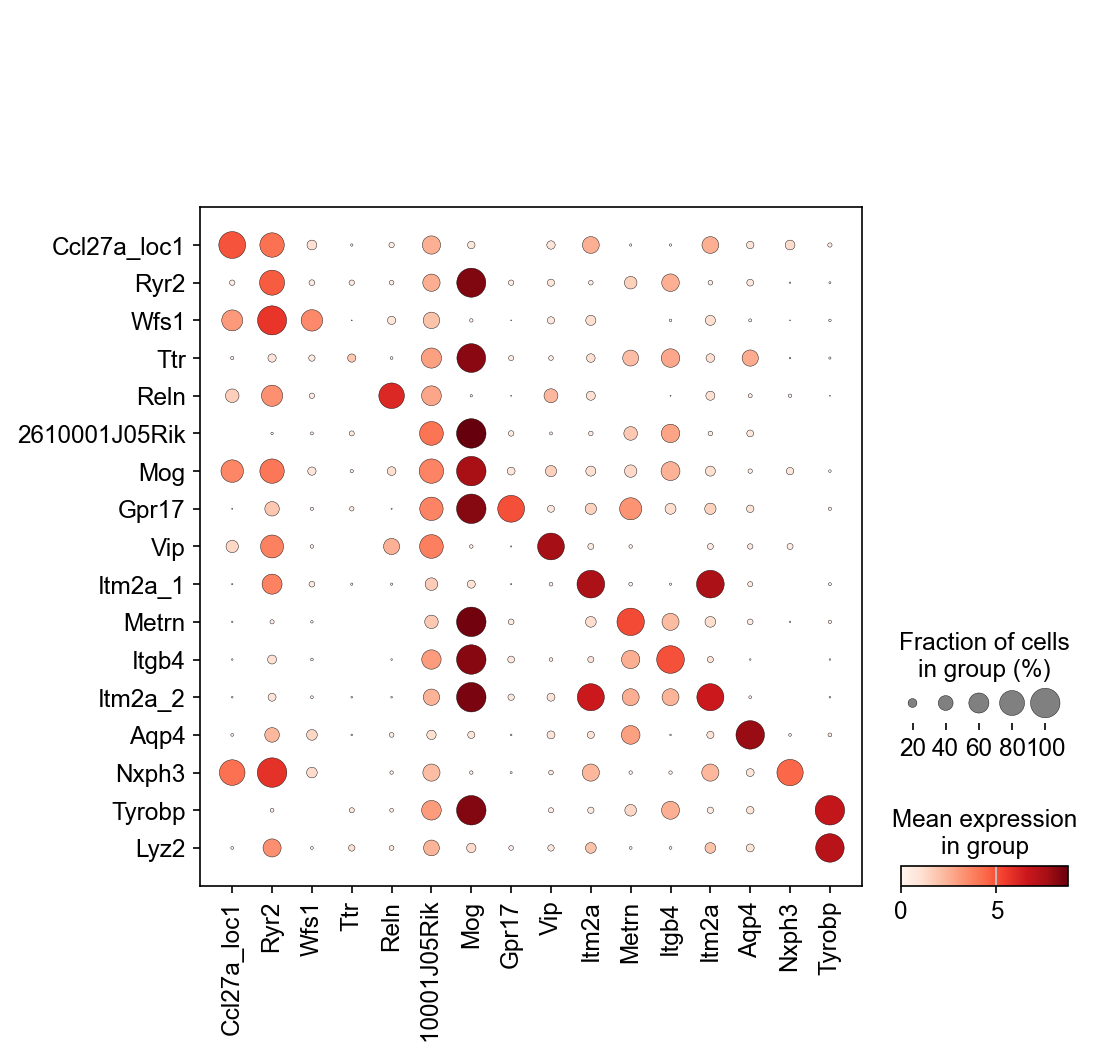
\includegraphics[width=4in,height=4in]{figures/fig6.png}
		\caption{标记基因气泡图}
	\end{figure}
	
	\begin{figure}[H]
		\centering
		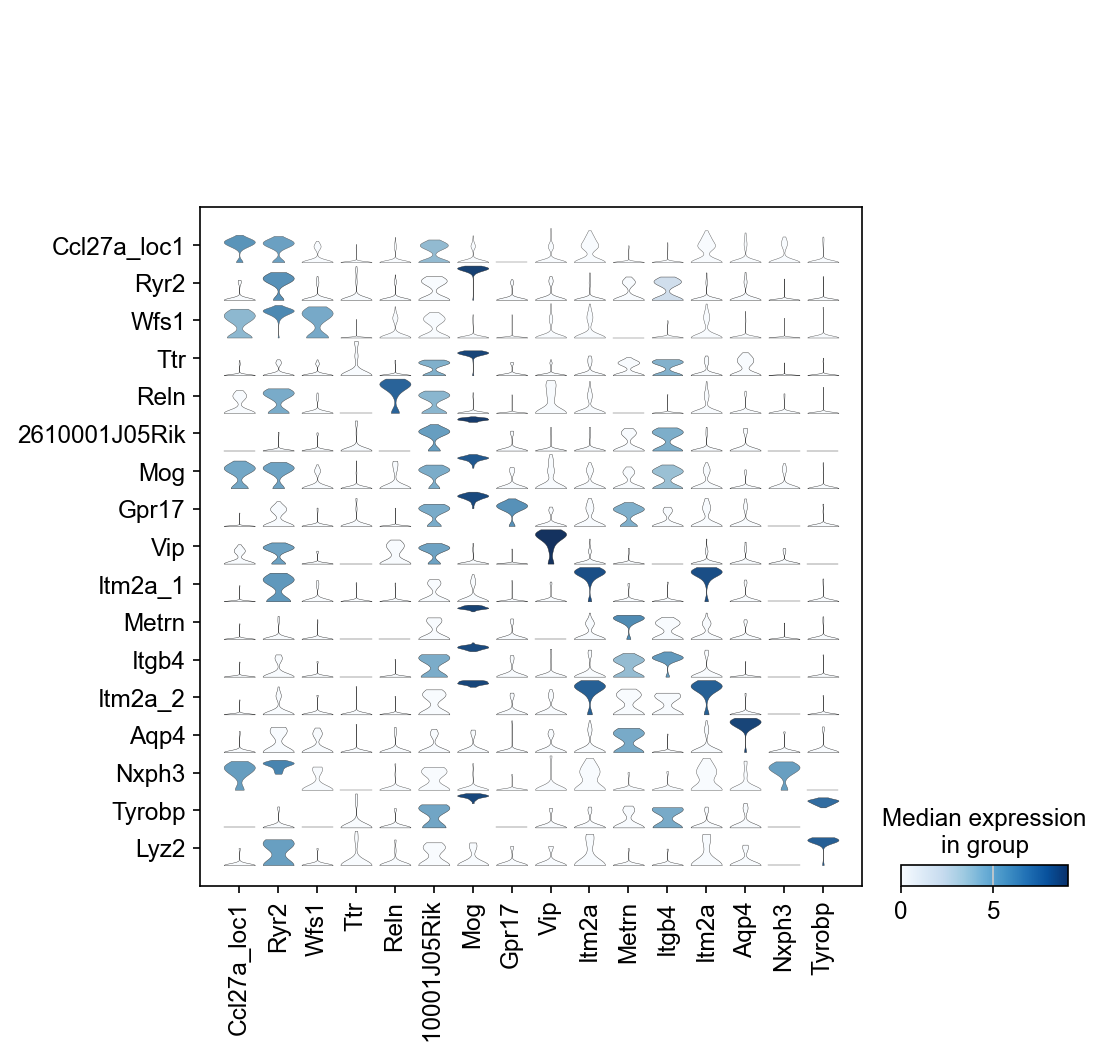
\includegraphics[width=3in,height=3in]{figures/fig7.png}
		\caption{标记基因小提琴图}
	\end{figure}
	
	聚类得分矩阵(标记细胞类型)的h5ad文件见实验结果目录。
	
	\section{结果分析}
	根据聚类指标的意义,可知聚类效果良好,总体准确性、聚类标签与真实标签的相似度较高。
	
	\section{实验讨论}
	\subsection{优缺点分析}
	本次实验过程有以下三点优点:
	\begin{itemize}
		\item 降维操作所用的主成分分析(PCA)算法是一种经典的线性降维算法,能够有效地捕捉数据中的主要变化方向,减少数据的维度并保留尽可能多的信息,且计算简单、易于理解;
		\item 聚类分析所用的Leiden算法是一种用于图聚类的优化算法,有着高效的聚类性能,支持重叠社区检测,自适应分辨率参数;
		\item 使用的模型算法具有鲁棒性、可迁移性,聚类结果准确合理。
	\end{itemize}
	
	不过,实验也存在以下两点缺点:
	\begin{itemize}
		\item 降维操作所用的主成分分析(PCA)算法假设数据是线性可分的,对于非线性关系的数据降维效果可能较差;
		\item 聚类分析所用的Leiden算法计算复杂度较高,没有明确的准则来指导参数的选择,对噪声和稀疏图较为敏感。
	\end{itemize}
	
	\subsection{改进方法}
	本次实验有以下两点可以进一步改进的方法:
	\begin{itemize}
		\item 降维操作可以选用对非线性关系数据也较为友好的方法;
		\item 聚类分析可以选用复杂度较低的方法。
	\end{itemize}
	
	\section{心得体会}
	做完本次实验,除了掌握了实验目的部分中所有内容的收获之外,我还有以下几点心得体会:
	\begin{itemize}
		\item 聚类分析前最好能先对数据进行降维;
		\item 得到聚类结果之后可以进一步计算每类的特征。
	\end{itemize}
	
	\section{参考文献}
	[1] Xiu Yan, 《清风数学建模学习笔记——主成分分析(PCA)原理详解及案例分析》, https://blog.csdn.net/weixin\_43819566/article/details/113800120
	
	[2] 无尽攀登, 《动手学单细胞分析-基础-2.5 聚类之Leiden》,https://zhuanlan.\\zhihu.com/p/538605686
	
	%\end{sloppypar}
\end{document}
\endinput